
%!TeX encoding = UTF-8
%!TeX program = xelatex
\documentclass[notheorems, aspectratio=54]{beamer}
% aspectratio: 1610, 149, 54, 43(default), 32

\usepackage{latexsym}
\usepackage{amsmath,amssymb}
\usepackage{mathtools}
\usepackage{color,xcolor}
\usepackage{graphicx}
\usepackage{algorithm}
\usepackage{amsthm}
\usepackage{lmodern} % 解决 font warning
% \usepackage[UTF8]{ctex}
\usepackage{animate} % insert gif

\usepackage{lipsum} % To generate test text 
\usepackage{ulem} % 下划线,波浪线

\usepackage{listings} % display code on slides; don't forget [fragile] option after \begin{frame}
% \usepackage{subcaption}
% ----------------------------------------------
% tikx
\usepackage{framed}
\usepackage{tikz}
\usepackage{pgf}
\usetikzlibrary{calc,trees,positioning,arrows,chains,shapes.geometric,%
    decorations.pathreplacing,decorations.pathmorphing,shapes,%
    matrix,shapes.symbols}
\pgfmathsetseed{1} % To have predictable results
% Define a background layer, in which the parchment shape is drawn
\pgfdeclarelayer{background}
\pgfsetlayers{background,main}

% define styles for the normal border and the torn border
\tikzset{
  normal border/.style={orange!30!black!10, decorate, 
     decoration={random steps, segment length=2.5cm, amplitude=.7mm}},
  torn border/.style={orange!30!black!5, decorate, 
     decoration={random steps, segment length=.5cm, amplitude=1.7mm}}}

% Macro to draw the shape behind the text, when it fits completly in the
% page
\def\parchmentframe#1{
\tikz{
  \node[inner sep=2em] (A) {#1};  % Draw the text of the node
  \begin{pgfonlayer}{background}  % Draw the shape behind
  \fill[normal border] 
        (A.south east) -- (A.south west) -- 
        (A.north west) -- (A.north east) -- cycle;
  \end{pgfonlayer}}}

% Macro to draw the shape, when the text will continue in next page
\def\parchmentframetop#1{
\tikz{
  \node[inner sep=2em] (A) {#1};    % Draw the text of the node
  \begin{pgfonlayer}{background}    
  \fill[normal border]              % Draw the ``complete shape'' behind
        (A.south east) -- (A.south west) -- 
        (A.north west) -- (A.north east) -- cycle;
  \fill[torn border]                % Add the torn lower border
        ($(A.south east)-(0,.2)$) -- ($(A.south west)-(0,.2)$) -- 
        ($(A.south west)+(0,.2)$) -- ($(A.south east)+(0,.2)$) -- cycle;
  \end{pgfonlayer}}}

% Macro to draw the shape, when the text continues from previous page
\def\parchmentframebottom#1{
\tikz{
  \node[inner sep=2em] (A) {#1};   % Draw the text of the node
  \begin{pgfonlayer}{background}   
  \fill[normal border]             % Draw the ``complete shape'' behind
        (A.south east) -- (A.south west) -- 
        (A.north west) -- (A.north east) -- cycle;
  \fill[torn border]               % Add the torn upper border
        ($(A.north east)-(0,.2)$) -- ($(A.north west)-(0,.2)$) -- 
        ($(A.north west)+(0,.2)$) -- ($(A.north east)+(0,.2)$) -- cycle;
  \end{pgfonlayer}}}

% Macro to draw the shape, when both the text continues from previous page
% and it will continue in next page
\def\parchmentframemiddle#1{
\tikz{
  \node[inner sep=2em] (A) {#1};   % Draw the text of the node
  \begin{pgfonlayer}{background}   
  \fill[normal border]             % Draw the ``complete shape'' behind
        (A.south east) -- (A.south west) -- 
        (A.north west) -- (A.north east) -- cycle;
  \fill[torn border]               % Add the torn lower border
        ($(A.south east)-(0,.2)$) -- ($(A.south west)-(0,.2)$) -- 
        ($(A.south west)+(0,.2)$) -- ($(A.south east)+(0,.2)$) -- cycle;
  \fill[torn border]               % Add the torn upper border
        ($(A.north east)-(0,.2)$) -- ($(A.north west)-(0,.2)$) -- 
        ($(A.north west)+(0,.2)$) -- ($(A.north east)+(0,.2)$) -- cycle;
  \end{pgfonlayer}}}

% Define the environment which puts the frame
% In this case, the environment also accepts an argument with an optional
% title (which defaults to ``Example'', which is typeset in a box overlaid
% on the top border
\newenvironment{parchment}[1][Example]{%
  \def\FrameCommand{\parchmentframe}%
  \def\FirstFrameCommand{\parchmentframetop}%
  \def\LastFrameCommand{\parchmentframebottom}%
  \def\MidFrameCommand{\parchmentframemiddle}%
  \vskip\baselineskip
  \MakeFramed {\FrameRestore}
  \noindent\tikz\node[inner sep=1ex, draw=black!20,fill=white, 
          anchor=west, overlay] at (0em, 2em) {\sffamily#1};\par}%
{\endMakeFramed}

% ----------------------------------------------

\mode<presentation>{
    \usetheme{CambridgeUS}
    % Boadilla CambridgeUS
    % default Antibes Berlin Copenhagen
    % Madrid Montpelier Ilmenau Malmoe
    % Berkeley Singapore Warsaw
    \usecolortheme{beaver}
    % beetle, beaver, orchid, whale, dolphin
    \useoutertheme{infolines}
    % infolines miniframes shadow sidebar smoothbars smoothtree split tree
    \useinnertheme{circles}
    % circles, rectanges, rounded, inmargin
}
% 设置 block 颜色
\setbeamercolor{block title}{bg=red!30,fg=white}

\newcommand{\reditem}[1]{\setbeamercolor{item}{fg=red}\item #1}

% 缩放公式大小
\newcommand*{\Scale}[2][4]{\scalebox{#1}{\ensuremath{#2}}}

% 解决 font warning
\renewcommand\textbullet{\ensuremath{\bullet}}

% ---------------------------------------------------------------------
% flow chart
\tikzset{
    >=stealth',
    punktchain/.style={
        rectangle, 
        rounded corners, 
        % fill=black!10,
        draw=white, very thick,
        text width=6em,
        minimum height=2em, 
        text centered, 
        on chain
    },
    largepunktchain/.style={
        rectangle,
        rounded corners,
        draw=white, very thick,
        text width=10em,
        minimum height=2em,
        on chain
    },
    line/.style={draw, thick, <-},
    element/.style={
        tape,
        top color=white,
        bottom color=blue!50!black!60!,
        minimum width=6em,
        draw=blue!40!black!90, very thick,
        text width=6em, 
        minimum height=2em, 
        text centered, 
        on chain
    },
    every join/.style={->, thick,shorten >=1pt},
    decoration={brace},
    tuborg/.style={decorate},
    tubnode/.style={midway, right=2pt},
    font={\fontsize{10pt}{12}\selectfont},
}
% ---------------------------------------------------------------------

% code setting
\lstset{
    language=C++,
    basicstyle=\ttfamily\footnotesize,
    keywordstyle=\color{red},
    breaklines=true,
    xleftmargin=2em,
    numbers=left,
    numberstyle=\color[RGB]{222,155,81},
    frame=leftline,
    tabsize=4,
    breakatwhitespace=false,
    showspaces=false,               
    showstringspaces=false,
    showtabs=false,
    morekeywords={Str, Num, List},
}

% ---------------------------------------------------------------------

%% preamble
\title[Multi-Agent RL]{Multi-Agent Reinforcement Learning}
% \subtitle{The subtitle}
\author{Yuxuan XIE}
\institute[HIT]{yuxuan.xie@hotmail.com}

% -------------------------------------------------------------

\begin{document}

%% title frame
\begin{frame}
  \titlepage
\end{frame}

%% normal frame
\begin{frame}
  \frametitle{Outline}

  \tableofcontents
  % \begin{itemize}
  %   \item Single Agent Reinforcement Learning
  %   \item Multi Agent RL and algorithms to solve
  %   \item Applications
  %   \item Current challenge
  % \end{itemize}
\end{frame}

\section{Single Agent Reinforcement Learning}
\begin{frame}
  \frametitle{The overview of RL}
  \vfill
  \begin{figure}[h]
    \begin{minipage}{0.45\textwidth}
      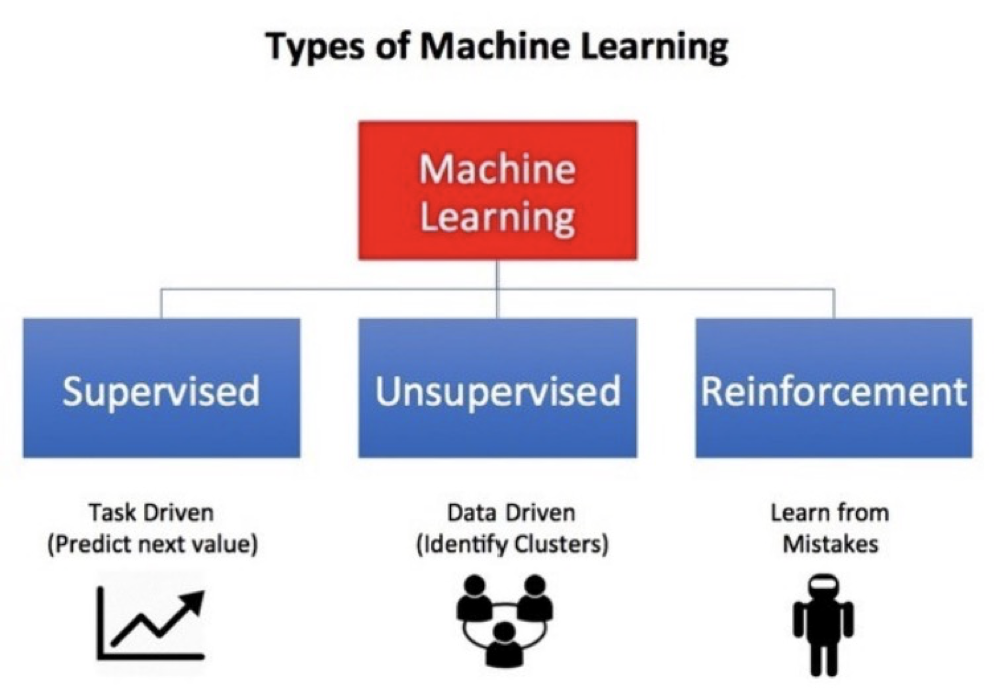
\includegraphics[width=\textwidth, height=5cm]{relation.png}
    \end{minipage}
    \hspace{0.05\linewidth}
    \begin{minipage}{0.45\textwidth}
      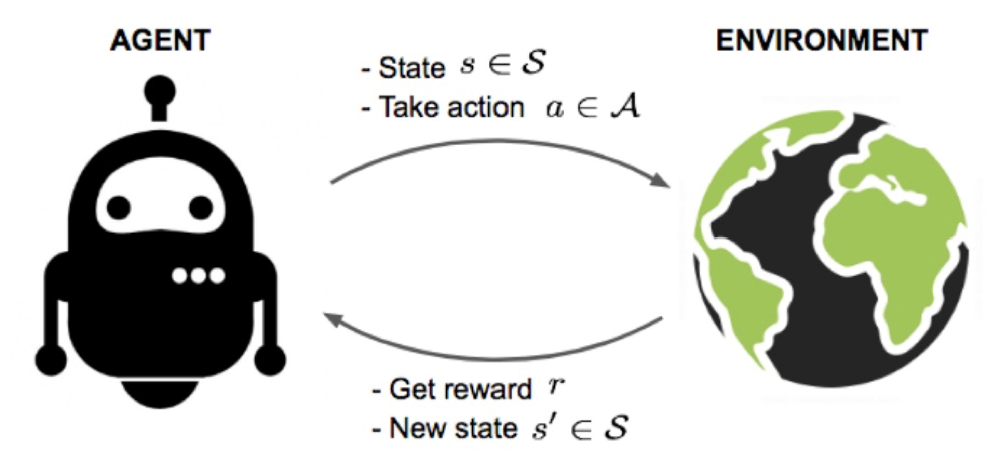
\includegraphics[width=\textwidth, height=3cm]{rl.png}
      Learning from interacting with the environment
    \end{minipage}
  \end{figure}
  \vfill
\end{frame}

\begin{frame}
  \frametitle{Why RL is so hot?}
  \centering
  \huge{\textbf{DL + RL = AGI}} \\
  \begin{flushright}
  \large{---David Silver}
  \end{flushright}
\end{frame}
\begin{frame}
  \frametitle{Markov Decision Process(MDP)}
  \begin{minipage}{0.45\textwidth}
    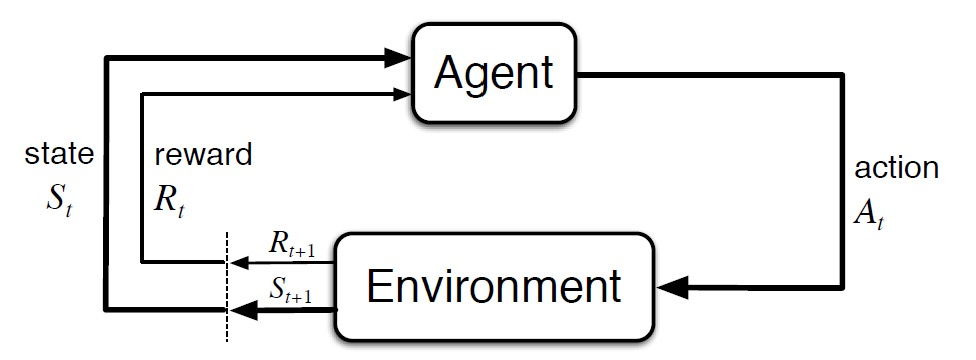
\includegraphics[width=\textwidth ]{mdp.png}
  \end{minipage}
  \hspace{0.05\linewidth}
  \begin{minipage}{0.45\textwidth}
  The MDP can be represented as a four element tuple $<S, A, R, P>$ 
  \begin{itemize}
    \item S : the set of state
    \item A : the set of action
    \item R : the set of reward
    \item P : the transition model
  \end{itemize}
  \end{minipage}

\end{frame}

\begin{frame}
  \frametitle{model-based and model-free}
  \textbf{Methods to solve model-based RL}
    \begin{itemize}
      \item Dynamic Programming
      \item Dyna(learn a model)
    \end{itemize}
  \textbf{Methods to solve model-free RL}
    \begin{itemize}
      \item Tabular based temporal-Difference Learning, e.g. Q-learning, SARSA
      \item Neural network based TD learning, e.g. DQN, DDQN
      \item Policy Gradient e.g. Actor-Critic, A3C, TRPO, PPO
    \end{itemize}
\end{frame}

\section{ Multi Agent RL and its challenges}
\begin{frame}
  \frametitle{Dec-POMDPs}
  \begin{minipage}{0.45\textwidth}
    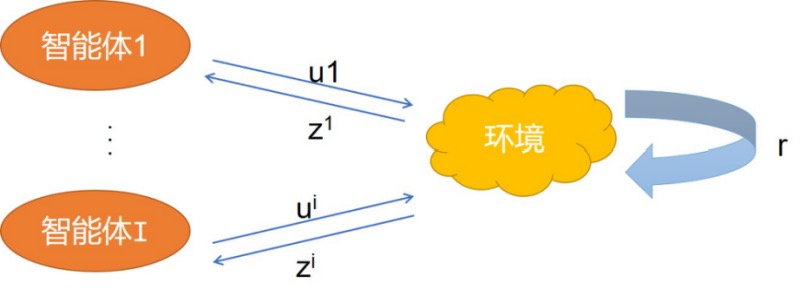
\includegraphics[width=\textwidth]{dec_pomdp.png}
  \end{minipage}
  \hspace{0.05\linewidth} 
  \begin{minipage}{0.45\textwidth}
    \begin{center}
    A $<S, A, R, P, O, N>$
    \end{center}
   \begin{itemize}
     \item S : the set of state
     \item A : the set of action $A = \times_{i}A^{i}$
     \item R : the set of reward 
     \item P : the transition model
     \item O : the set of observation $O = \times_{i}O^{i}$
     \item N : the number of agent
   \end{itemize}
  
  \end{minipage}
  \end{frame}


\section{Methods to solve but not optimally}
\begin{frame}
  \frametitle{Model-based and Model-free}
  \textbf{Methods to solve model-based RL}
  \begin{itemize}
    \item Counterfactural regret minimazition (CFR)
    \item Occupancy-belief-state-HSVI 
  \end{itemize}
  
  \textbf{Methods to solve model-free RL}
    \begin{itemize}
      \item[] core mechanism : Centralizd trainning and decentralized execution
      \begin{itemize}
        \item Value based : IQL, VDN, QMIX, QTRAN,  
        \item Policy based : COMA, MADDPG
      \end{itemize}
    \end{itemize}

\end{frame}

\begin{frame}
  \frametitle{Independent Q-Learning}
  \begin{center}
    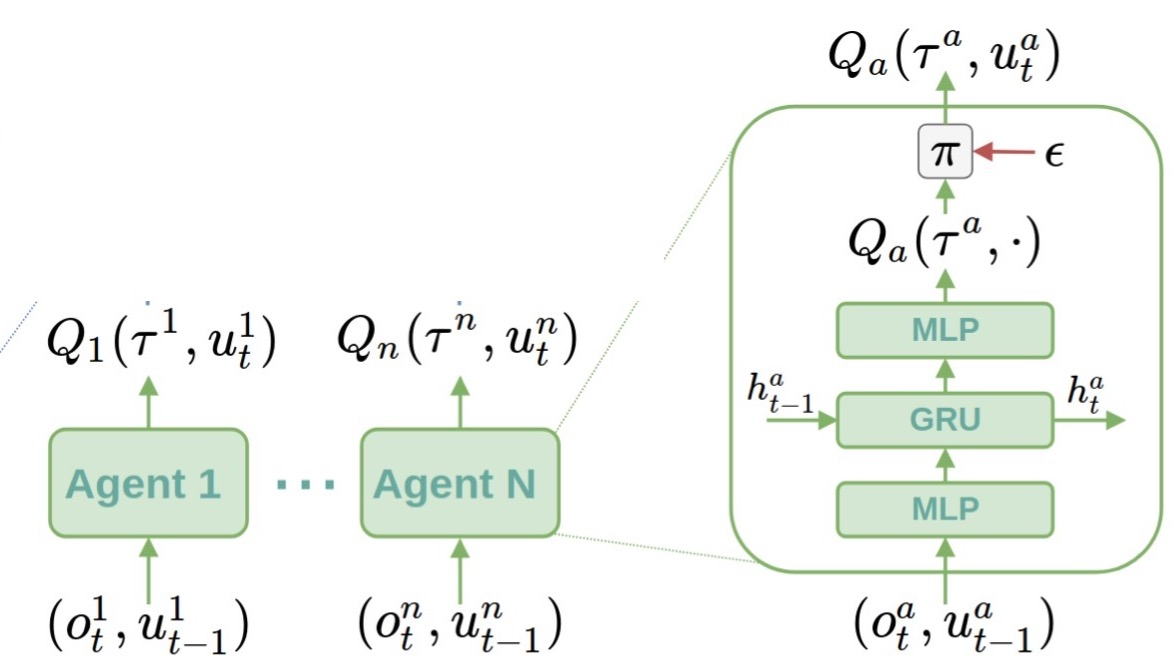
\includegraphics[width=0.8\textwidth]{IQL.png}
  \end{center}
  Every agent makes their own decision and others are treated as the environment. Then the environment is dynamic.
\end{frame}

\begin{frame}
  \frametitle{VDN and QMIX}
  \begin{center}
    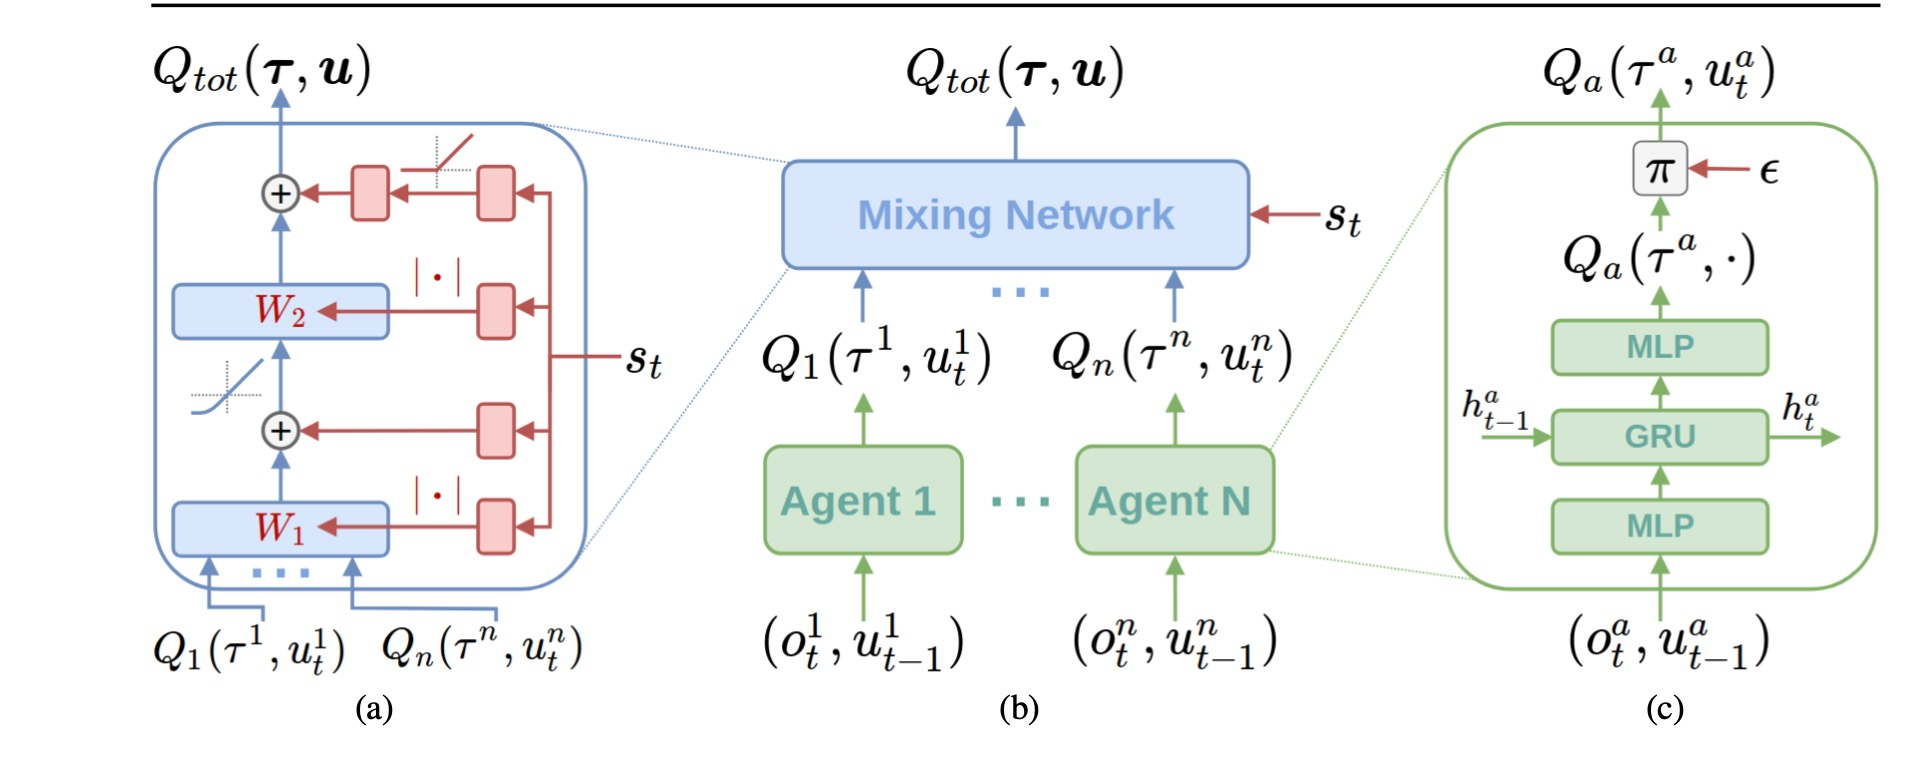
\includegraphics[width=0.8\textwidth]{QMIX.png}
  \end{center}
    The mix network just works during the trainning process.\\
    For VDN its a sum operator. \\
\end{frame}

\begin{frame}
  \frametitle{COMA}
  \begin{center}
    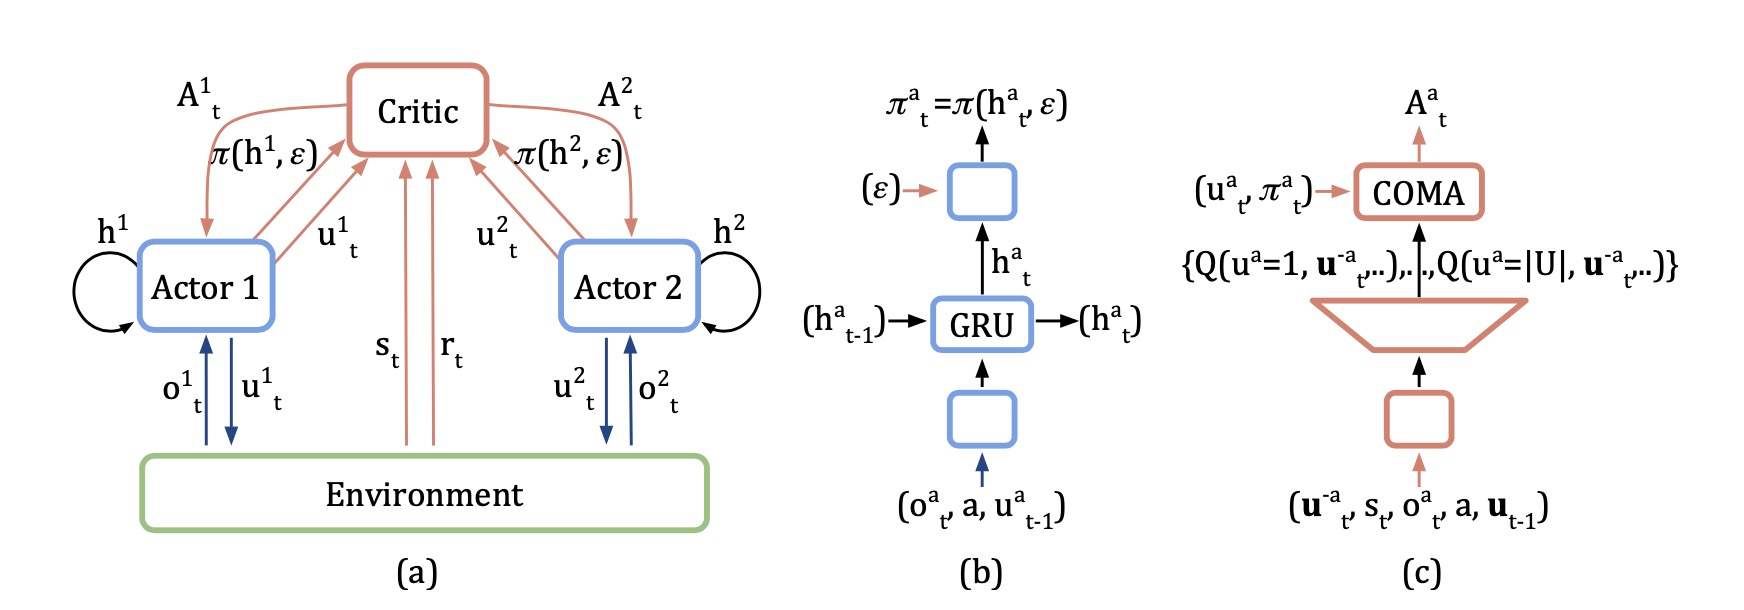
\includegraphics[width=0.8\textwidth]{coma.png}
  \end{center}
\end{frame}

\section{Applications}
\begin{frame}
  \vfill
  \begin{figure}[h]
  \begin{minipage}{0.45\textwidth}
    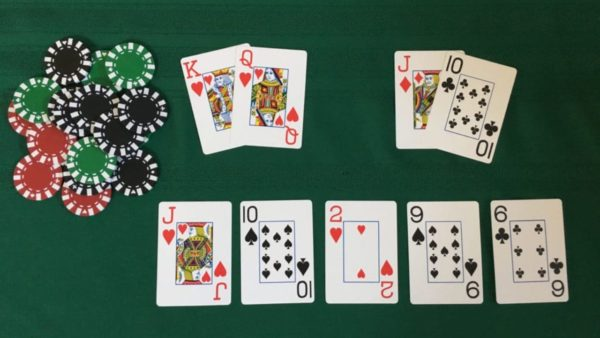
\includegraphics[width=\textwidth]{holdem-showdown-1280x720-600x338.jpg}
    \begin{center}
    Teaxs hold'em
    \end{center}
  \end{minipage}%
  \hspace{0.02\linewidth}
  \begin{minipage}{0.45\textwidth}
    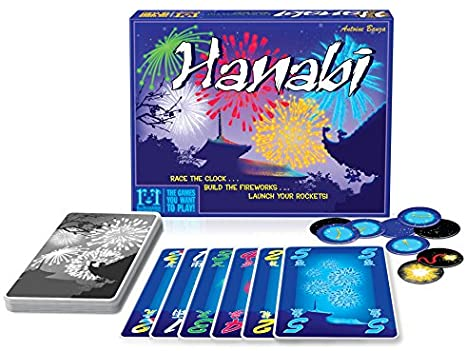
\includegraphics[width=\textwidth]{hanabi.jpg}
    \begin{center}
    Hanabi
    \end{center}
    \end{minipage}
  \begin{minipage}{0.45\textwidth}
    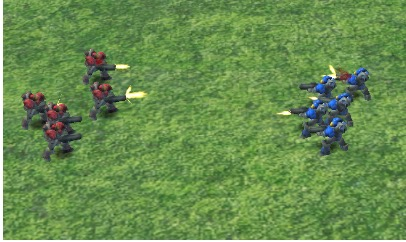
\includegraphics[width=\textwidth]{ starcraft.png}
    \begin{center}
    Starcraft
    \end{center}
  \end{minipage}
  \hspace{0.02\linewidth}
  \begin{minipage}{0.45\textwidth}
    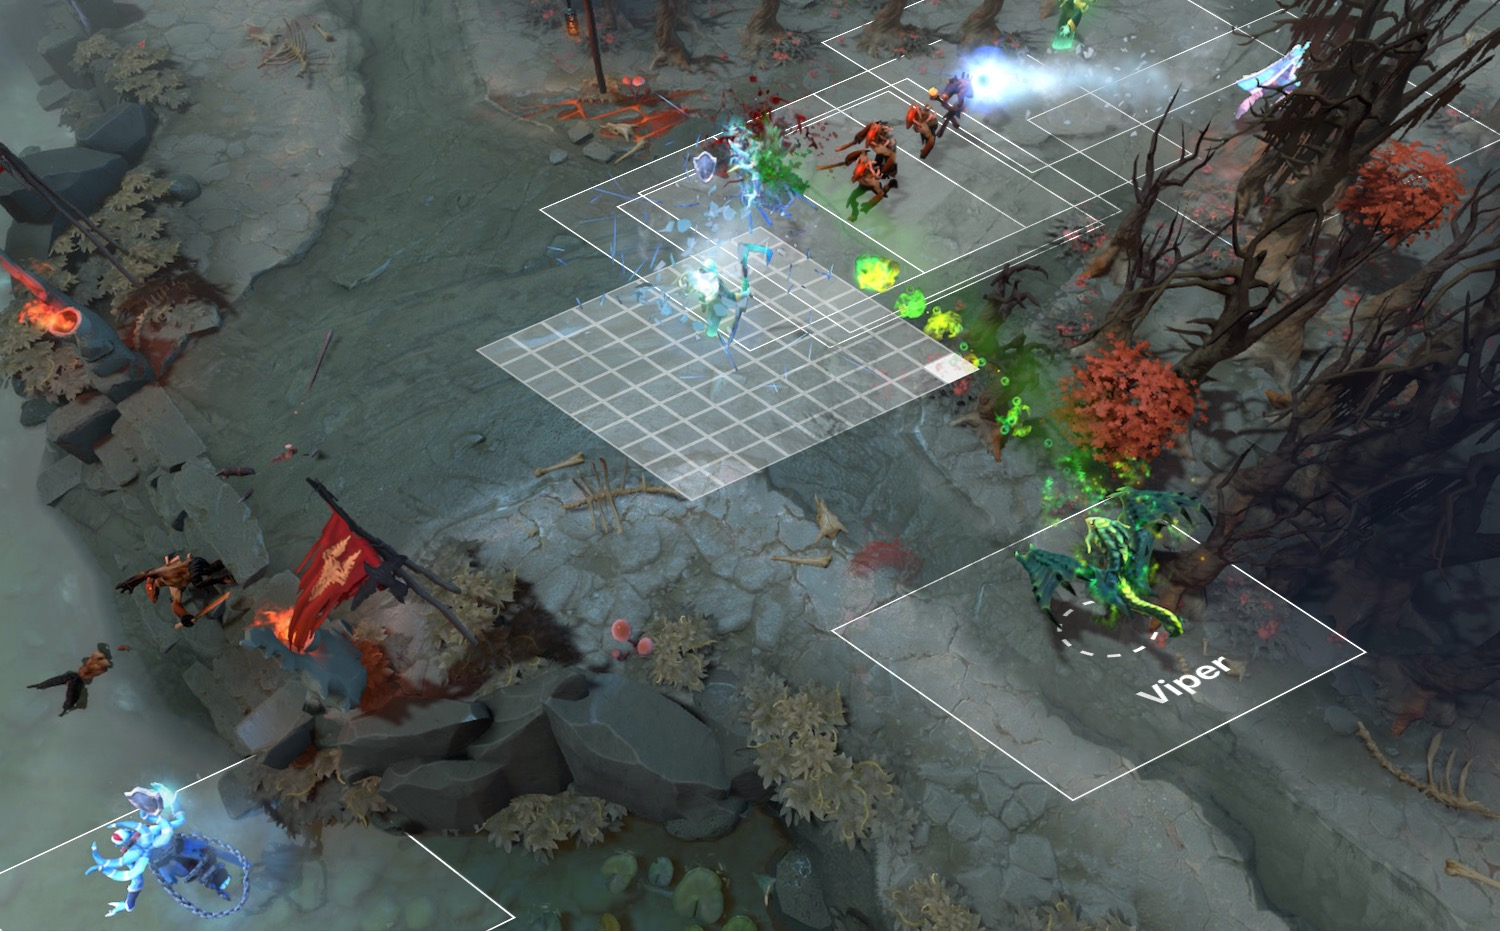
\includegraphics[width=\textwidth]{ dota.png}
    \begin{center}
    dota 
    \end{center}
  \end{minipage}
  \end{figure}
  \vfill
  
\end{frame}

\end{document}
